\section*{Background}
JSS is an optimization problem in CS and operation research, and it can be extended to many different problem depend on the given “constraints”. In this document, we will follow the Google Project’s version[2]: Suppose there are many jobs which are processed by several machines, Job shop scheduling problem is to minimize the length of the schedule under the following constraints:

\begin{enumerate}
 \item Each job consists of a sequence of tasks, which must be performed in a given order

  \item Each task must be processed on a specific(correspond) machine

   \item No task can be started until the previous task is completed

    \item A machine can only work on one task at one time

     \item Once a machine start a task, it need to run to complete


\end{enumerate}
Here is the example from Google’s project: Each task below is labeled by a pair of numbers (m, p) where m is the number of the machine the task must be processed on and p is the processing time of the task — the amount of time it requires. (The numbering of jobs and machines starts at 0.)
\begin{itemize}
\item job 0 = [(0, 3), (1, 2), (2, 2)]
\item job 1 = [(0, 2), (2, 1), (1, 4)]
\item job 2 = [(1, 4), (2, 3)]
\end{itemize}

\begin{figure}[H]
\centering
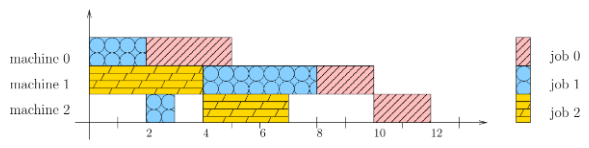
\includegraphics[width=4in]{img/1.PNG}
\caption{one possible solution for Google JSS example}
\end{figure}